\chapter{Описание стенда и подготовка}
\label{ch:stand}

\section{Конфигурация виртуального стенда}

Для выполнения работы используются три виртуальные машины из предыдущих
лабораторных работ~5--8:

\begin{itemize}
  \item \textbf{gateway} — Ubuntu~20.04.5~LTS Server, два адаптера:
        \texttt{enp0s3}~(NAT, \texttt{10.0.2.15/24}),
        \texttt{enp0s8}~(Internal, \texttt{192.168.\cfgLabStudentN.1/24}).
        Роль: Ansible control node, DNS, DHCP.
  \item \textbf{desktop1} — Ubuntu~20.04.5~Desktop, адаптер
        Internal~(\texttt{192.168.\cfgLabStudentN.10}). Роль: Ansible client~1.
  \item \textbf{wordpress} — Ubuntu~20.04.5~LTS Server,\\адаптер
        Internal~(\texttt{192.168.\cfgLabStudentN.6}). Роль: Ansible client~2.
\end{itemize}

% --- Скриншот: ip a на gateway (все интерфейсы) ---
\begin{figure}[h]
  \centering
  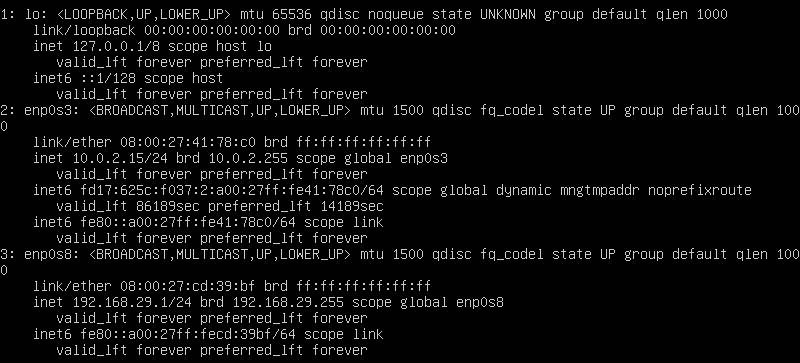
\includegraphics{img/01_gateway_ip_a}
  \caption{Сетевые интерфейсы ВМ \texttt{gateway} — вывод \texttt{ip a}}
  \label{fig:gateway_ip_a}
\end{figure}

\section{Подготовка клиентских ВМ}

На каждой клиентской ВМ (\texttt{desktop1} и \texttt{wordpress})
необходимо установить \texttt{openssh-server} и \texttt{python3},
а также запустить SSH в автозагрузку.
Для этого запускается скрипт \texttt{client\_lab9\_prepare.sh}:

\begin{lstlisting}
sudo bash client_lab9_prepare.sh
\end{lstlisting}

Скрипт выполняет:
\begin{enumerate}
  \item \texttt{apt-get update} — обновление списка пакетов;
  \item \texttt{apt-get install -y openssh-server python3};
  \item \texttt{systemctl enable ssh \&\& systemctl start ssh}.
\end{enumerate}

% --- Скриншот: systemctl status ssh на desktop1 ---
\begin{figure}[h]
  \centering
  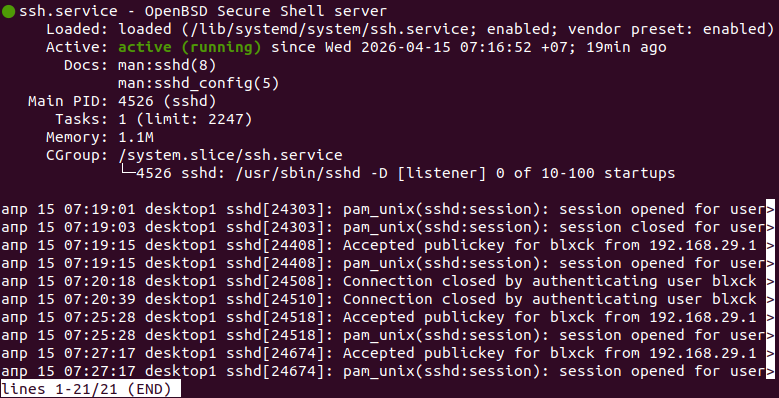
\includegraphics{img/02_client_ssh_status}
  \caption{Статус службы SSH на клиентской ВМ \texttt{desktop1}}
  \label{fig:client_ssh_status}
\end{figure}

% --- Скриншот: systemctl status ssh на wordpress ---
\begin{figure}[h]
  \centering
  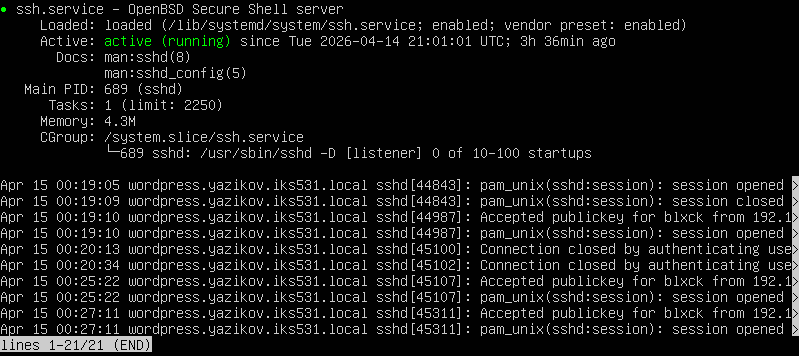
\includegraphics{img/03_wordpress_ssh_status}
  \caption{Статус службы SSH на клиентской ВМ \texttt{wordpress}}
  \label{fig:wordpress_ssh_status}
\end{figure}

\section{Проверка сетевой связности}

Перед установкой Ansible проверяется доступность клиентов с gateway:

\begin{lstlisting}
ping -c 3 192.168.29.10
ping -c 3 192.168.29.6
\end{lstlisting}

% --- Скриншот: ping desktop1 и wordpress с gateway ---
\begin{figure}[h]
  \centering
  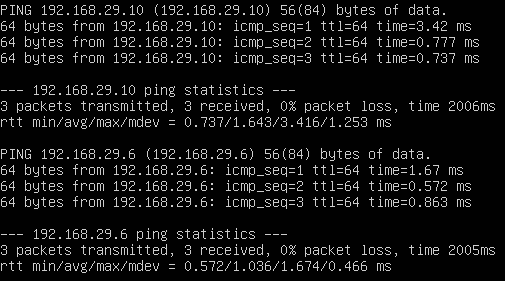
\includegraphics{img/04_ping_clients}
  \caption{Проверка связности с клиентами с ВМ \texttt{gateway}}
  \label{fig:ping_clients}
\end{figure}

\endinput
